% Titre de la premiere partie
\section[Intro]{Introduction Historique}

%%%%%%%%%%%%%%%%%%%%%%%%%%%%%%%%%%%%%%%%%%%%%%%%
% Première diapo
%%%%%%%%%%%%%%%%%%%%%%%%%%%%%%%%%%%%%%%%%%%%%%%%
\begin{frame}
	\frametitle{Introduction historique}
	\framesubtitle{Position du problème}

	\begin{block}{Un peu d'histoire}
		La mécanique newtonienne, une mécanique bien huilée
	\end{block}

	\pause

	\begin{alertblock}{Le problème du périhélie de Mercure}
		\pause
		\begin{figure}
			\visible<+->{
				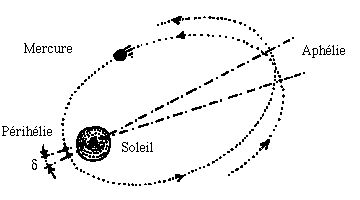
\includegraphics[width=0.6\linewidth]{figures/Fig01}
				\caption{Précession du périhélie de Mercure}
			}
		\end{figure}
	\end{alertblock}

\end{frame}


%%%%%%%%%%%%%%%%%%%%%%%%%%%%%%%%%%%%%%%%%%%%%%%%
% Deuxième diapo
%%%%%%%%%%%%%%%%%%%%%%%%%%%%%%%%%%%%%%%%%%%%%%%%
\begin{frame}
	\frametitle{Introduction historique}
	\framesubtitle{Explication classique}

	\begin{columns}
		\column{0.5\linewidth} % première colonne
			Plusieurs explications en compétitions:

			\pause

			\begin{itemize}[<+->]
				\item		Théorie des perturbations: explication de $531''$ d'arc/siècle
				\item		Vulcain, un bon candidat (Le Verrier, 1859)
				\item		mais pas de confirmation expérimentale...

			\end{itemize}



		\column{0.5\linewidth} % 2e colonne
			\begin{alertblock}{Ça ne va pas}<+->
				Il manque un élément à la théorie!
			\end{alertblock}

	\end{columns}

\end{frame}


%%%%%%%%%%%%%%%%%%%%%%%%%%%%%%%%%%%%%%%%%%%%%%%%
% Troisième diapo
%%%%%%%%%%%%%%%%%%%%%%%%%%%%%%%%%%%%%%%%%%%%%%%%
\begin{frame}
	\frametitle{Introduction historique}
	\framesubtitle{Complément relativiste}

	\begin{block}{L'avis de la relativité restreinte}
		$7''$ d'arc
		en plus par siècle
	\end{block}

	\pause

	\begin{exampleblock}{La générale sauve la mise}
		Rajoute
		les $43''$ qui manquaient.
	\end{exampleblock}

\end{frame}
